\chapter*{Results}
\label{ch:results}
The performance metrics considered for evaluation in these analysis are the following: accuracy, precision,
recall, and F1-score. The latter one is the harmonic mean of precision and recall and was therefore chosen for further discussion in this section. Considering all of these metrics is crucial to accurately evaluate how well each
model performs.
Regarding the static models implemented in this project, the classification report revealed an accuracy of
34\% for the Random Forest algorithm and 43\% for SVM. These results can be considered reasonable, given that the task at hand is a multi-class classification problem with 8 classes.\\

For the Random Forest model, the class with the highest F1-score is \texttt{anger}, which is the third class as for support, sitting at 4436. 
\texttt{Joy} was the most supported class, with 5854 instances, but it came second as for the F1-score, which was of 0.40. The second class based off support, which was \texttt{fear} with 4652 instances, had a lower F1-score of 0.31. 
The remaining classes showed comparable support and F1-scores, averaging around 3500 instances and 0.25 respectively, only \texttt{disgust} had a considerably lower F1-score, at 18\%. \\
In image \ref{fig:roc_rf}, the ratio of true positives versus false positives is displayed, with the Random Forest classifier scoring lower than a random guesser in two out of eight classes. \\
\begin{figure}[H]
    \centering
    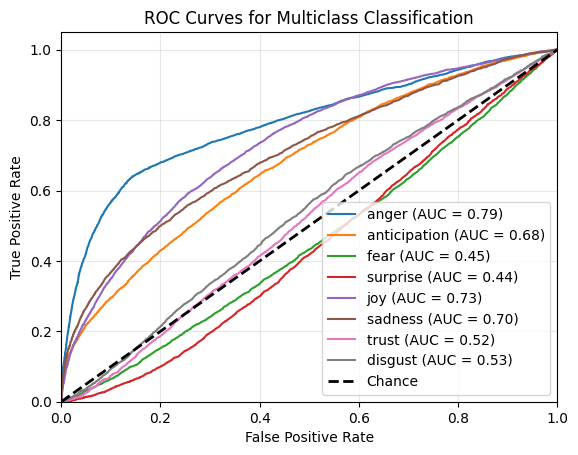
\includegraphics[width=0.5\linewidth]{pictures/roc_rf.png}
    \caption{ROC Curve for the Random Forest Classifier}
    \label{fig:roc_rf}
\end{figure}
Image \textbf{DA AGGIUNGERE IMMAGINE} shows class-wise accuracy. \\

\textbf{DA AGGIUNGERE SVM}\\

Neural Networks' performances were generally not on par with the ones obtained by
the static models.
As mentioned in the previous chapter, the development of neural networks
iterated testing phases and adjustments over different configurations for data
splitting, preprocessing, architectures and training parameters were tested.
Because of the generally poor results, semi-supervised learning did not get
important results; downsampling into evenly represented labels gave some
minor improvements, for both architectures.\\

The graphs below show various performance metrics of the best network for the
convolutional architecture.
\begin{figure}[H]
    \centering
    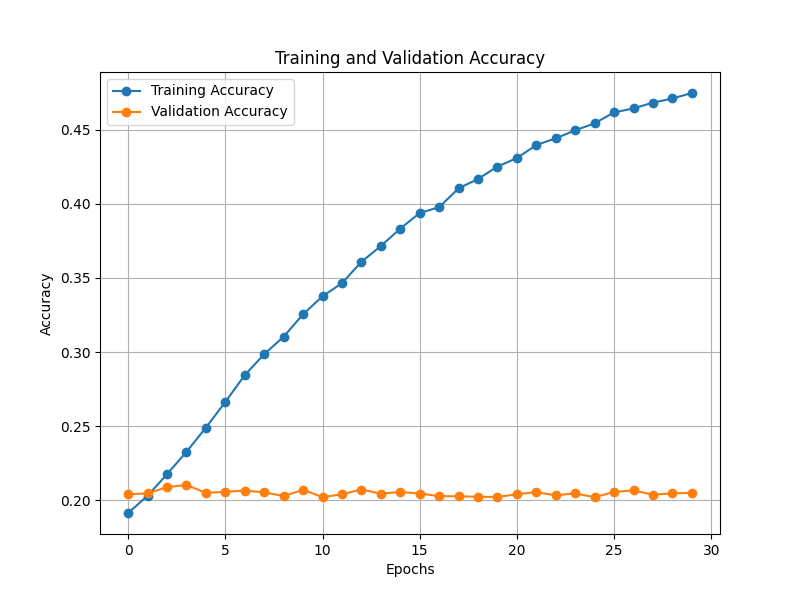
\includegraphics[width=0.7\linewidth]{pictures/cnn_accuracy.png}
    \caption{Convolutional Neural Network's training and validation accuracy}
    \label{fig:cnn_train_val_acc}
\end{figure}

\begin{figure}[H]
    \centering
    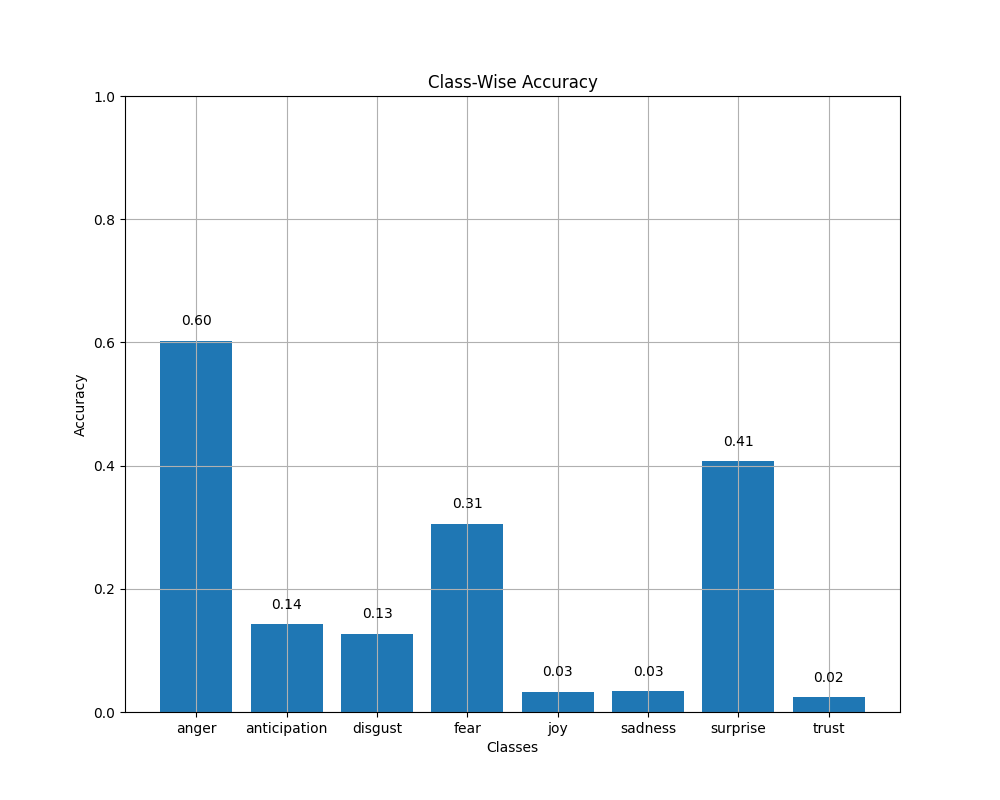
\includegraphics[width=0.7\linewidth]{pictures/cnn_class_accuracy.png}
    \caption{Convolutional Neural Network's class-wide accuracy}
    \label{fig:cnn_classacc}
\end{figure}

\begin{figure}[H]
    \centering
    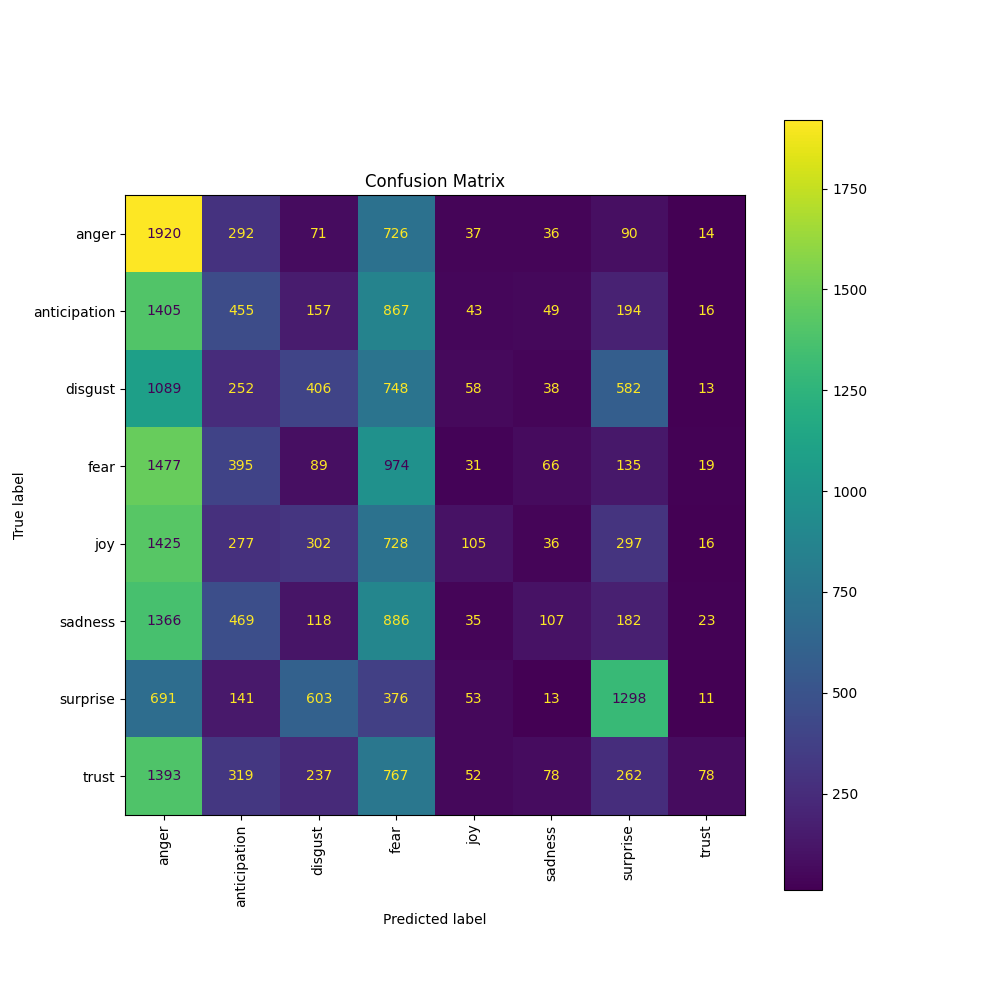
\includegraphics[width=0.7\linewidth]{pictures/cnn_confusion_matrix.png}
    \caption{Convolutional Neural Network's confusion matrix}
    \label{fig:cnn_confmatr}
\end{figure}

% Judging from the confusion matrices
% and training and validation accuracy plots, the models tend to confuse the classes.
% This might be because of heavy high frequency overlapping terms between the classes